% Strategy Pipeline — Concept Diagram
% Compile with: pdflatex strategy-pipeline.tex
\documentclass[border=14pt]{standalone}

\usepackage[T1]{fontenc}
\usepackage[english]{babel}
\usepackage{lmodern}
\usepackage{amsmath}
\usepackage{xcolor}
\usepackage{tikz}
\usetikzlibrary{
    decorations.pathmorphing,
    decorations.pathreplacing,
    arrows.meta,
    positioning,
    calc,
    shapes.geometric,
    backgrounds,
    fit
}

%% ---------- Colour palette ----------
\definecolor{ink}        {HTML}{1F2433}
\definecolor{soft}       {HTML}{9CA3AF}
\definecolor{nodebg}     {HTML}{F4F6FA}
\definecolor{accent}     {HTML}{3A6E5B}  % distillate / key flow
\definecolor{lens}       {HTML}{C8553D}  % source cloud / "MORE ACTION!"
\definecolor{lensbg}     {HTML}{FBEBE6}
\definecolor{phase1}     {HTML}{4A6FA5}  % Concept
\definecolor{phase1bg}   {HTML}{EBF1F9}
\definecolor{phase2}     {HTML}{C9883A}  % Coaching / Implementation
\definecolor{phase2bg}   {HTML}{FBF2DD}
\definecolor{phase3}     {HTML}{4F8A6B}  % Integration
\definecolor{phase3bg}   {HTML}{E7F0EA}
\definecolor{execborder} {HTML}{C8CFDB}
\definecolor{execbg}     {HTML}{FBFCFE}

\begin{document}
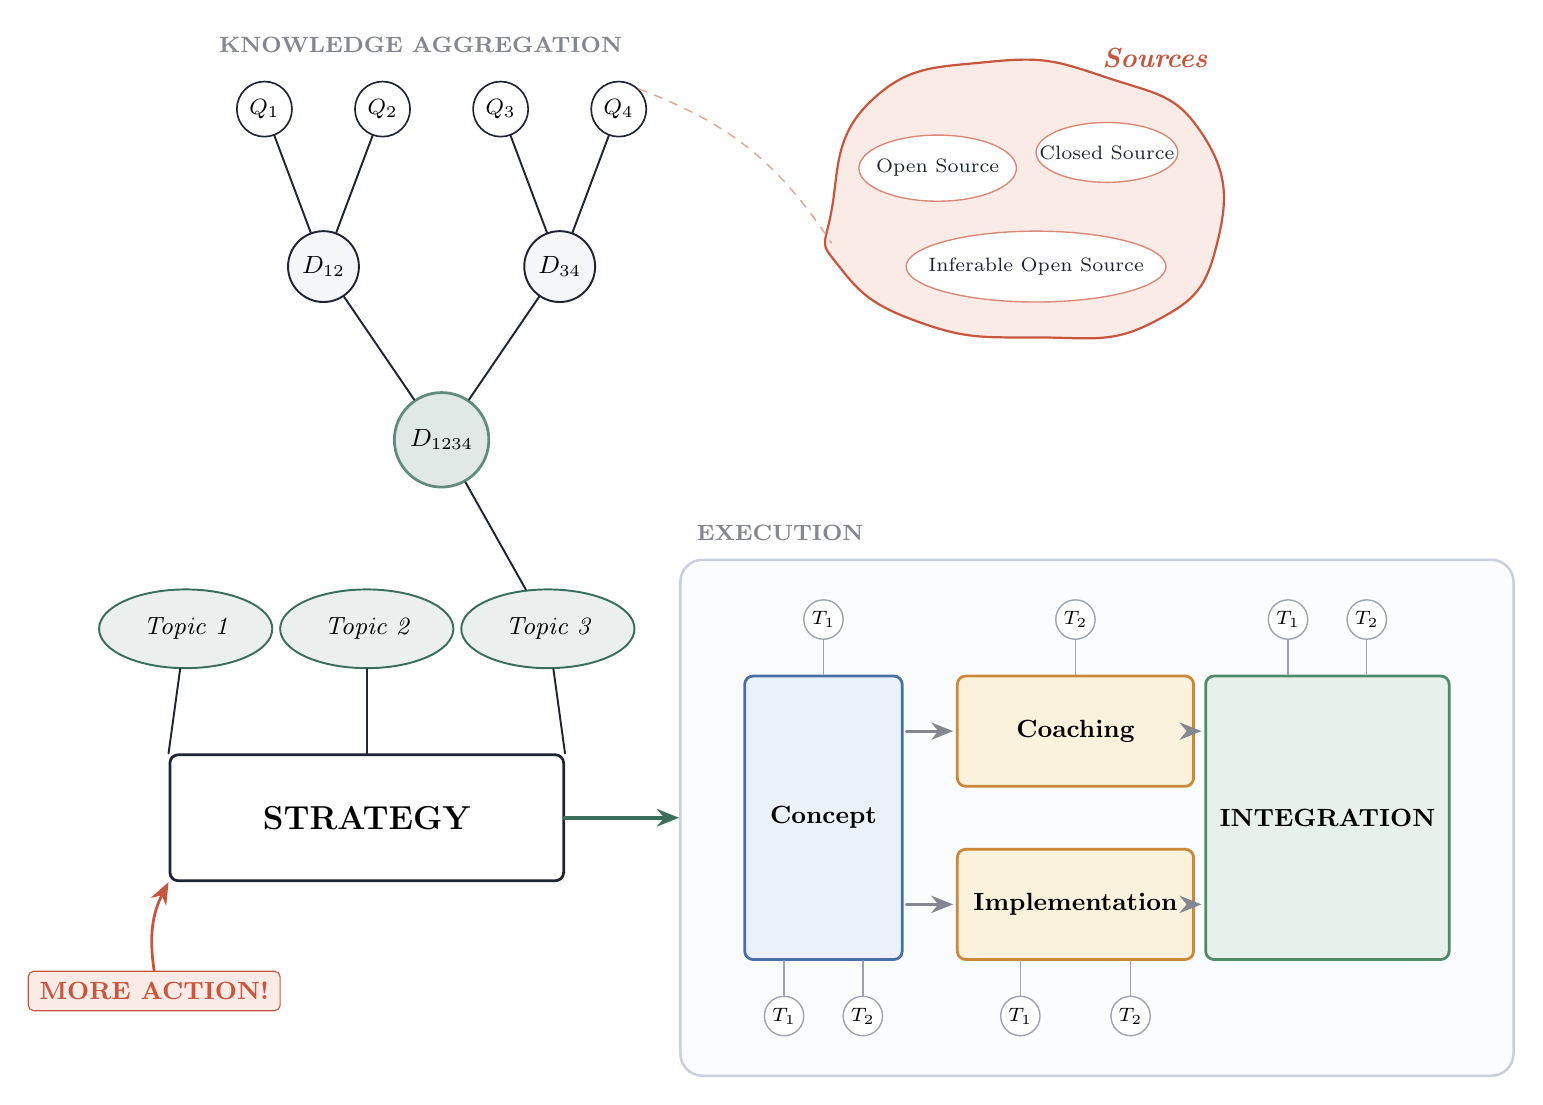
\begin{tikzpicture}[
    line cap=round, line join=round,
    >={Stealth[length=2.8mm, width=2.2mm]},
    %% --- semantic styles ---
    outline/.style      = {draw=ink, line width=0.7pt},
    thinline/.style     = {draw=soft, line width=0.5pt},
    qnode/.style        = {circle, draw=ink, line width=0.6pt, fill=white,
                           minimum size=7mm, inner sep=1pt, font=\footnotesize},
    dnode/.style        = {circle, draw=ink, line width=0.7pt, fill=nodebg,
                           minimum size=9mm, inner sep=1pt, font=\small},
    rootnode/.style     = {circle, draw=accent!80, line width=1pt, fill=accent!15,
                           minimum size=12mm, inner sep=1pt, font=\small},
    topic/.style        = {ellipse, draw=accent, fill=accent!10, line width=0.7pt,
                           minimum width=22mm, minimum height=10mm,
                           font=\small\itshape},
    sbox/.style         = {rectangle, draw=ink, fill=white, line width=1pt,
                           rounded corners=3pt, minimum width=50mm,
                           minimum height=16mm, font=\large\bfseries,
                           align=center},
    pbox/.style         = {rectangle, draw=ink!85, fill=white, line width=0.9pt,
                           rounded corners=3pt, font=\small\bfseries,
                           align=center, inner sep=5pt},
    keyflow/.style      = {->, draw=accent, line width=1.6pt},
    procflow/.style     = {->, draw=ink!55, line width=1pt,
                           shorten >=1pt, shorten <=1pt},
    tinynode/.style     = {circle, draw=soft, line width=0.5pt, fill=white,
                           minimum size=5mm, inner sep=0pt, font=\scriptsize},
    sectionlabel/.style = {font=\footnotesize\bfseries, text=ink!55},
    callout/.style      = {font=\small\bfseries, text=lens, draw=lens,
                           fill=lensbg, rounded corners=2pt, inner sep=4pt}
]

%% ================================================================
%% TOP-LEFT — Knowledge aggregation tree
%% ================================================================
\node[qnode] (Q1) at (-4.0, 8.0) {$Q_1$};
\node[qnode] (Q2) at (-2.5, 8.0) {$Q_2$};
\node[qnode] (Q3) at (-1.0, 8.0) {$Q_3$};
\node[qnode] (Q4) at ( 0.5, 8.0) {$Q_4$};

\node[dnode] (D12)   at (-3.25, 6.0) {$D_{12}$};
\node[dnode] (D34)   at (-0.25, 6.0) {$D_{34}$};
\node[rootnode] (D1234) at (-1.75, 3.8) {$D_{1234}$};

\foreach \a/\b in {Q1/D12, Q2/D12, Q3/D34, Q4/D34, D12/D1234, D34/D1234}
    \draw[outline] (\a) -- (\b);

\node[sectionlabel, anchor=south west] at (-4.7, 8.6)
    {KNOWLEDGE AGGREGATION};

%% ================================================================
%% TOP-RIGHT — Source taxonomy cloud
%% ================================================================
\begin{scope}[shift={(5.6, 6.7)}]
    \draw[lens, fill=lensbg, line width=0.8pt]
        plot[smooth cycle, tension=0.85] coordinates {
            (-2.4,  0.0) (-1.9,  1.4) (-0.4,  1.9) ( 1.1,  1.7)
            ( 2.3,  1.0) ( 2.5, -0.4) ( 1.7, -1.4) ( 0.2, -1.6)
            (-1.3, -1.4) (-2.3, -0.7)
        };
    \node[font=\itshape\bfseries, text=lens, anchor=south east]
        at (2.5, 1.7) {Sources};

    \draw[lens!70, line width=0.5pt, fill=white]
        (-1.05, 0.55) ellipse (1.00 and 0.42);
    \node[font=\scriptsize, text=ink] at (-1.05, 0.55) {Open Source};

    \draw[lens!70, line width=0.5pt, fill=white]
        ( 1.10, 0.75) ellipse (0.90 and 0.38);
    \node[font=\scriptsize, text=ink] at ( 1.10, 0.75) {Closed Source};

    \draw[lens!70, line width=0.5pt, fill=white]
        ( 0.20, -0.70) ellipse (1.65 and 0.45);
    \node[font=\scriptsize, text=ink] at ( 0.20, -0.70) {Inferable Open Source};
\end{scope}

% subtle hint that Q's are drawn from the source pool
\draw[dashed, lens!55, line width=0.5pt]
    (Q4.north east) to[bend left=18]
    ($(5.6, 6.7) + (-2.4, -0.4)$);

%% ================================================================
%% MIDDLE — Topics → STRATEGY
%% ================================================================
\node[topic] (Top1) at (-5.0, 1.4) {Topic 1};
\node[topic] (Top2) at (-2.7, 1.4) {Topic 2};
\node[topic] (Top3) at (-0.4, 1.4) {Topic 3};

\draw[outline] (D1234) -- (Top3);

\node[sbox] (STRAT) at (-2.7, -1.0) {STRATEGY};
\draw[outline] (Top1) -- (STRAT.north west);
\draw[outline] (Top2) -- (STRAT.north);
\draw[outline] (Top3) -- (STRAT.north east);

%% ================================================================
%% RIGHT — EXECUTION container with process flow
%% ================================================================
% Phase 1 — Concept (tall left bar)
\node[pbox, fill=phase1bg, draw=phase1, line width=1pt,
      minimum width=20mm, minimum height=36mm]
    (CONCEPT) at (3.1, -1.0) {Concept};

% Phase 2 — parallel streams (Coaching above, Implementation below)
\node[pbox, fill=phase2bg, draw=phase2, line width=1pt,
      minimum width=30mm, minimum height=14mm]
    (COACH) at (6.3, 0.1) {Coaching};
\node[pbox, fill=phase2bg, draw=phase2, line width=1pt,
      minimum width=30mm, minimum height=14mm]
    (IMPL)  at (6.3, -2.1) {Implementation};

% Phase 3 — Integration (tall right bar)
\node[pbox, fill=phase3bg, draw=phase3, line width=1pt,
      minimum width=22mm, minimum height=36mm,
      font=\small\bfseries]
    (INTEG) at (9.5, -1.0) {INTEGRATION};

% --- Internal process flow arrows ---
\draw[procflow] (CONCEPT.east |- COACH.west) -- (COACH.west);
\draw[procflow] (CONCEPT.east |- IMPL.west)  -- (IMPL.west);
\draw[procflow] (COACH.east)  -- (INTEG.west |- COACH.east);
\draw[procflow] (IMPL.east)   -- (INTEG.west |- IMPL.east);

% --- T markers as inputs (above each phase) ---
\node[tinynode] (Tc_in)  at ($(CONCEPT.north) + (0,    7mm)$) {$T_1$};
\node[tinynode] (Tco_in) at ($(COACH.north)   + (0,    7mm)$) {$T_2$};
\node[tinynode] (Ti1_in) at ($(INTEG.north)   + (-5mm, 7mm)$) {$T_1$};
\node[tinynode] (Ti2_in) at ($(INTEG.north)   + ( 5mm, 7mm)$) {$T_2$};

\draw[thinline] (Tc_in)  -- (CONCEPT.north);
\draw[thinline] (Tco_in) -- (COACH.north);
\draw[thinline] (Ti1_in) -- ($(INTEG.north) + (-5mm, 0)$);
\draw[thinline] (Ti2_in) -- ($(INTEG.north) + ( 5mm, 0)$);

% --- T markers as outputs (below) ---
\node[tinynode] (Tc1_out) at ($(CONCEPT.south) + (-5mm, -7mm)$) {$T_1$};
\node[tinynode] (Tc2_out) at ($(CONCEPT.south) + ( 5mm, -7mm)$) {$T_2$};
\node[tinynode] (Tu1_out) at ($(IMPL.south)    + (-7mm, -7mm)$) {$T_1$};
\node[tinynode] (Tu2_out) at ($(IMPL.south)    + ( 7mm, -7mm)$) {$T_2$};

\draw[thinline] ($(CONCEPT.south) + (-5mm, 0)$) -- (Tc1_out);
\draw[thinline] ($(CONCEPT.south) + ( 5mm, 0)$) -- (Tc2_out);
\draw[thinline] ($(IMPL.south)    + (-7mm, 0)$) -- (Tu1_out);
\draw[thinline] ($(IMPL.south)    + ( 7mm, 0)$) -- (Tu2_out);

% --- Container box (background layer, auto-fitted) ---
\begin{scope}[on background layer]
    \node[draw=execborder, fill=execbg, rounded corners=8pt,
          line width=0.9pt,
          inner xsep=8mm, inner ysep=5mm,
          fit=(CONCEPT) (COACH) (IMPL) (INTEG)
              (Tc_in) (Tco_in) (Ti1_in) (Ti2_in)
              (Tc1_out) (Tc2_out) (Tu1_out) (Tu2_out)]
          (EXECBOX) {};
\end{scope}

% Container title
\node[sectionlabel, anchor=south west]
    at ($(EXECBOX.north west) + (1mm, 1mm)$) {EXECUTION};

% --- Key arrow: STRATEGY → EXECUTION ---
\draw[keyflow] (STRAT.east) -- (EXECBOX.west |- STRAT.east);

%% ================================================================
%% "MORE ACTION!" sticky-note callout
%% ================================================================
\node[callout] (MA) at (-5.4, -3.2) {MORE ACTION!};
\draw[->, lens, line width=1pt]
    (MA.north) to[bend left=18] (STRAT.south west);

\end{tikzpicture}
\end{document}
